\documentclass[conference]{IEEEtran}
\IEEEoverridecommandlockouts

\usepackage{cite}
\usepackage{amsmath,amssymb,amsfonts}
\usepackage{graphicx}
\usepackage{textcomp}
\usepackage{xcolor}
\usepackage{booktabs}
\usepackage{pifont}
\usepackage{url}
\usepackage{tikz}
\usetikzlibrary{positioning,arrows.meta,fit,backgrounds,calc}

\graphicspath{{figures/}}
\newcommand{\yes}{\ding{51}}
\newcommand{\no}{\ding{55}}
\newcommand{\pt}{$\sim$}
\newcommand{\vect}[1]{\mathbf{#1}}

% Places IEEE author blocks on a second row.
\makeatletter
\newcommand{\linebreakand}{%
  \end{@IEEEauthorhalign}
  \hfill\mbox{}\par
  \mbox{}\hfill\begin{@IEEEauthorhalign}
}
\makeatother

\begin{document}

\title{RehabSense: A Low-Cost Bilateral Wearable System with Mounting-Invariant Activity Recognition for ACL Rehabilitation Monitoring}

\author{
\IEEEauthorblockN{Yash Trivedi}
\IEEEauthorblockA{\textit{Dept. of Computer Engineering} \\
\textit{Vishwakarma Institute of Technology}\\
Pune, India \\
trivediyash154@gmail.com}
\and
\IEEEauthorblockN{Darshil Zade}
\IEEEauthorblockA{\textit{Dept. of Computer Engineering} \\
\textit{Vishwakarma Institute of Technology}\\
Pune, India}
\and
\IEEEauthorblockN{Tejal Sapkale}
\IEEEauthorblockA{\textit{Dept. of Computer Engineering} \\
\textit{Vishwakarma Institute of Technology}\\
Pune, India}
\linebreakand
\IEEEauthorblockN{Yukta Myadam}
\IEEEauthorblockA{\textit{Dept. of Computer Engineering} \\
\textit{Vishwakarma Institute of Technology}\\
Pune, India}
\and
\IEEEauthorblockN{Naina Kokate}
\IEEEauthorblockA{\textit{Dept. of Computer Engineering} \\
\textit{Vishwakarma Institute of Technology}\\
Pune, India}
}

\maketitle

\begin{abstract}
Recovery after anterior cruciate ligament (ACL) reconstruction is judged largely by between-limb symmetry, yet objective movement assessment remains confined to laboratories. Low-cost inertial wearables could extend monitoring into daily rehabilitation, but models that assume a fixed sensor orientation break when patients re-attach the straps. We present RehabSense, an end-to-end research platform built around a US\$18 wearable in which one ESP32 samples an MPU6050 inertial measurement unit on each shank and two heel force sensors on a single 100\,Hz clock, with an integrity-checked streaming protocol, a per-wearing eight-check calibration and a cloud analytics service. We propose a mounting-invariant representation that combines orientation-invariant inertial channels with posture measured against the calibrated neutral pose, and select the activity model by a rule fixed before any results were seen. Under subject-independent evaluation on real bilateral public data, the deployed random forest reaches a macro-F1 of 0.921 that is unchanged under random sensor re-mounting, whereas raw-axis features collapse from 0.943 to 0.199; inference takes 12.9\,ms per window (95th percentile). Device-format replay reproduces the training pipeline on 98.4\% of windows, and transparent asymmetry and Movement Quality Index metrics respond monotonically to injected deficits in simulation. A cross-dataset test (macro-F1 0.15--0.24) quantifies the domain gap that the forthcoming on-device pilot study must close.
\end{abstract}

\begin{IEEEkeywords}
anterior cruciate ligament, wearable sensors, inertial measurement unit, human activity recognition, orientation invariance, limb symmetry, random forest, Internet of Things
\end{IEEEkeywords}

% =====================================================================
\section{Introduction}

Return to sport after ACL reconstruction is a symmetry decision: patients who returned before passing objective criteria, including a limb symmetry index of at least 90\%, were reinjured far more often~\cite{grindem2016}. Yet symmetry is measured objectively only in laboratories~\cite{tan2023}, so most of a recovery lasting nine months or more goes unobserved. Remote programmes already match brochure-based home rehabilitation on early outcomes~\cite{lim2024}, but they rarely measure how the patient moves.

Inertial measurement units (IMUs) are the most common portable modality for ACL assessment, yet recent scoping reviews find most systems at technology readiness levels 3--6, with calibration and criterion validation reported inconsistently and few demonstrations outside the laboratory~\cite{tan2023,ptaszyk2025}. We identify three obstacles. (i)~\emph{Mounting}: estimators and activity models that assume a fixed sensor orientation degrade when the strap is re-attached, which at home happens every session~\cite{yurtman2017,baek2026}. (ii)~\emph{Evaluation}: record-wise splits inflate accuracy~\cite{saeb2017}, and public-dataset scores are presented as if they transfer to new hardware despite well-documented domain shift~\cite{hong2024,napoli2024}. (iii)~\emph{Transparency}: composite ``recovery scores'' combine components with unexplained weights.

RehabSense is designed around these obstacles. Its contributions are:
\begin{enumerate}
\item a low-cost bilateral node in which one ESP32 reads both shank IMUs and the force sensors in the same 100\,Hz tick, with a protocol and integrity layer that make loss, jitter, drift and sensor failure explicit rather than imputed;
\item a mounting-invariant representation that keeps posture by measuring it against a calibrated neutral pose, and a segment-tilt estimator whose rotation axis is learned from the calibration movement;
\item a subject-independent benchmark over three public datasets with device-specific robustness tests, and a model-selection rule fixed before results were observed;
\item transparent asymmetry and Movement Quality Index (MQI) metrics that never impute missing inputs, with evidence levels (public data, simulation, hardware, clinical) kept separate in the software.
\end{enumerate}
Sections~II--VII present related work, the system, the methods, the experimental setup, the results and the limitations.

% =====================================================================
\section{Related Work and Research Gap}

\subsection{Wearable Sensing after ACL Reconstruction}
Reviews of 49 out-of-lab ACL studies~\cite{tan2023} and 32 wearable studies~\cite{ptaszyk2025} found few systems validated outside the laboratory and none integrated into care. Phan et~al.~\cite{phan2026} monitored 26 patients with five IMUs for up to a week and observed inter-limb knee-extension asymmetry falling from 7.7$^\circ$ to 2.6$^\circ$ between three and nine months, a change the laboratory captured only partly---evidence that free-living symmetry monitoring adds information. Seel et~al.~\cite{seel2014} estimated knee angles without assuming sensor orientation by identifying the joint axis from motion. Low-cost ESP32 designs estimate knee flexion from thigh and shank MPU6050s~\cite{korbel2026}, add force sensors and a cloud back end for symmetry indices~\cite{joshita2026}, or fuse IMUs at the edge with 3.1--6.4$^\circ$ RMSE against video~\cite{achmamad2025}.

\subsection{Orientation- and Domain-Robust Activity Recognition}
Yurtman and Barshan~\cite{yurtman2017} removed absolute orientation by transforming raw signals; Gil-Mart\'{\i}n et~al.~\cite{gilmartin2023} mapped signals into a consistent reference frame; Barua et~al.~\cite{barua2024} used heuristic invariant features; and Baek et~al.~\cite{baek2026}, motivated by at-home re-attachment, built invariance to per-location rotations into an SO(3)-equivariant network. Invariance, however, discards the segment's posture, which is what separates sitting from standing. Cross-dataset generalisation remains hard even with self-supervised pretraining~\cite{hong2024,napoli2024}; CNN and CNN-LSTM networks~\cite{ordonez2016} are the standard deep baselines.

\begin{table}[t]
\caption{Representative approaches and the gap RehabSense addresses}
\label{tab:gap}
\centering
\scriptsize
\setlength{\tabcolsep}{2.6pt}
\begin{tabular}{@{}lcccccc@{}}
\toprule
Approach & Cost & \shortstack{Out-of-\\lab} & \shortstack{Sync.\\bilat.} & \shortstack{Mount.\\robust} & \shortstack{Activity\\model$^\dagger$} & \shortstack{Transp.\\metrics} \\
\midrule
Lab mocap / force plates~\cite{tan2023} & High & \no & \yes & -- & \no & \yes \\
Free-living multi-IMU~\cite{phan2026} & Med. & \yes & \yes & \pt & \no & \pt \\
Low-cost knee wearables~\cite{korbel2026,joshita2026,achmamad2025} & Low & \yes & \pt & \pt & \no & \pt \\
Invariant HAR~\cite{yurtman2017,gilmartin2023,baek2026} & -- & -- & \no & \yes & \yes & \no \\
\textbf{RehabSense (ours)} & \textbf{Low} & \yes & \yes & \yes & \yes & \yes \\
\bottomrule
\end{tabular}\\[2pt]
\parbox{\columnwidth}{\scriptsize \yes~addressed; \pt~partial or system-dependent; \no~not addressed; --~not applicable. $^\dagger$Learned activity model evaluated subject-independently.}
\end{table}

\subsection{Research Gap}
Low-cost knee wearables concentrate on single-joint angles, while orientation-robust activity recognition has been developed on public datasets without rehabilitation metrics (Table~\ref{tab:gap}). To our knowledge, no low-cost system combines (a)~synchronous bilateral capture, (b)~mounting-invariant activity recognition that keeps posture, (c)~subject-independent, pre-registered evaluation that measures its own domain gap, and (d)~movement metrics whose components and missing inputs are explicit.

% =====================================================================
\begin{figure*}[t]
\centering
% System architecture (Fig. 1). Requires tikz libraries: positioning, arrows.meta, fit, backgrounds, calc.
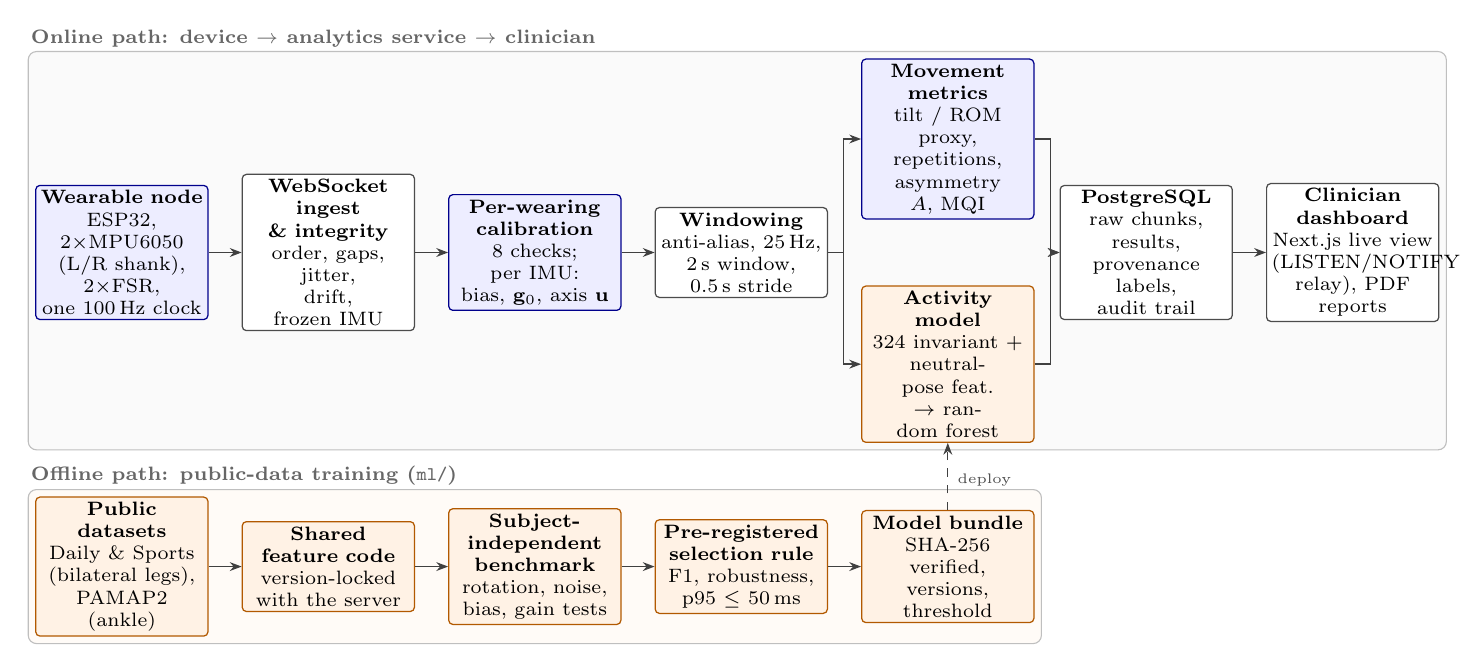
\begin{tikzpicture}[
  font=\scriptsize,
  >={Stealth[length=1.5mm]},
  box/.style={draw=black!70, rounded corners=1.5pt, align=center, inner sep=1.8pt,
              minimum height=8.4mm, text width=20.6mm, fill=white, line width=0.45pt},
  key/.style={box, fill=blue!7, draw=blue!55!black},
  ml/.style={box, fill=orange!10, draw=orange!70!black},
  lane/.style={draw=black!25, rounded corners=3pt, fill=black!2, inner xsep=2.5pt, inner ysep=2.5pt},
  lanelabel/.style={font=\scriptsize\bfseries, text=black!60, anchor=south west, inner sep=1pt},
  flow/.style={->, line width=0.5pt, draw=black!75},
  node distance=2mm and 4.2mm
]
% ---------------- online path (top lane)
\node[key] (dev) {\textbf{Wearable node}\\ESP32, 2$\times$MPU6050\\(L/R shank), 2$\times$FSR,\\one 100\,Hz clock};
\node[box, right=of dev] (ing) {\textbf{WebSocket ingest}\\\textbf{\& integrity}\\order, gaps, jitter,\\drift, frozen IMU};
\node[key, right=of ing] (cal) {\textbf{Per-wearing}\\\textbf{calibration}\\8 checks; per IMU:\\bias, $\mathbf{g}_0$, axis $\mathbf{u}$};
\node[box, right=of cal] (win) {\textbf{Windowing}\\anti-alias, 25\,Hz,\\2\,s window,\\0.5\,s stride};
\node[key, above right=-1.6mm and 4.2mm of win] (ana) {\textbf{Movement metrics}\\tilt / ROM proxy,\\repetitions,\\asymmetry $A$, MQI};
\node[ml, below right=-1.6mm and 4.2mm of win] (har) {\textbf{Activity model}\\324 invariant +\\neutral-pose feat.\\$\rightarrow$ random forest};
\node[box, right=29.4mm of win] (db) {\textbf{PostgreSQL}\\raw chunks, results,\\provenance labels,\\audit trail};
\node[box, right=of db] (ui) {\textbf{Clinician dashboard}\\Next.js live view\\(LISTEN/NOTIFY\\relay), PDF reports};

\draw[flow] (dev) -- (ing);
\draw[flow] (ing) -- (cal);
\draw[flow] (cal) -- (win);
\draw[flow] (win.east) -- ++(2mm,0) |- (ana.west);
\draw[flow] (win.east) -- ++(2mm,0) |- (har.west);
\draw[flow] (ana.east) -- ++(2mm,0) |- (db.west);
\draw[flow] (har.east) -- ++(2mm,0) |- (db.west);
\draw[flow] (db) -- (ui);

% ---------------- offline path (bottom lane)
\path (har.south) ++(0,-6.8mm) coordinate (offy);
\node[ml, anchor=north] (pub) at (dev.center |- offy) {\textbf{Public datasets}\\Daily \& Sports\\(bilateral legs),\\PAMAP2 (ankle)};
\node[ml, right=of pub] (feat) {\textbf{Shared feature code}\\version-locked\\with the server};
\node[ml, right=of feat] (cv) {\textbf{Subject-independent}\\\textbf{benchmark}\\rotation, noise,\\bias, gain tests};
\node[ml, right=of cv] (sel) {\textbf{Pre-registered}\\\textbf{selection rule}\\F1, robustness,\\p95 $\le$ 50\,ms};
\node[ml, right=of sel] (bun) {\textbf{Model bundle}\\SHA-256 verified,\\versions, threshold};
\draw[flow] (pub) -- (feat);
\draw[flow] (feat) -- (cv);
\draw[flow] (cv) -- (sel);
\draw[flow] (sel) -- (bun);
\draw[flow, dashed] (bun.north) -- (bun.north |- har.south) node[pos=0.45, right, font=\tiny, text=black!70]{deploy};

\begin{scope}[on background layer]
  \node[lane, fit=(dev)(ing)(cal)(win)(har)(ana)(db)(ui)] (online) {};
  \node[lane, fill=orange!3, fit=(pub)(feat)(cv)(sel)(bun)] (offline) {};
\end{scope}
\node[lanelabel] at (online.north west) {Online path: device $\rightarrow$ analytics service $\rightarrow$ clinician};
\node[lanelabel] at (offline.north west) {Offline path: public-data training (\texttt{ml/})};
\end{tikzpicture}

\caption{RehabSense architecture. Online: the node streams synchronised bilateral samples; the service checks stream integrity, calibrates every wearing, windows the signals and runs the activity model and movement metrics; results reach the dashboard through a PostgreSQL relay. Offline: models are benchmarked on public data with the same feature code the server runs, selected by a pre-registered rule and deployed as hash-verified bundles.}
\label{fig:arch}
\end{figure*}

\section{System Architecture}

\subsection{Wearable Node}
Fig.~\ref{fig:arch} shows the online and offline paths. An ESP32 DevKit~V1 reads two GY-521 MPU6050 IMUs, strapped to the lateral left and right shanks, over one I$^2$C bus at 400\,kHz; the AD0 pin selects address 0x68 (left) or 0x69 (right) (Fig.~\ref{fig:hw}). Each IMU is set to $\pm4$\,g and $\pm500^\circ$/s with its low-pass filter at about 44\,Hz, and the configuration is read back at boot. Two FSR402 heel sensors form 10\,k$\Omega$ dividers on ADC1 pins (ADC2 is unusable while Wi-Fi is active); their output is reported as a normalised ADC value, an uncalibrated \emph{load proxy}, never as newtons. An 18650 cell feeds a TP4056 charger and an MT3608 boost converter set to 5\,V. The parts cost about INR~1{,}560 (US\$18) at Indian retail prices.

A FreeRTOS task on core~1 wakes on a fixed period, reads both IMUs and the force channels in the same tick, stamps them with one microsecond timestamp and queues them in a lock-free ring buffer; the main loop sends ten samples per WebSocket frame (optionally over TLS). A failed read is sent as \texttt{null}, never as the previous or the other side's value, and status frames report ring overflows and I$^2$C errors so that device-side loss can be told apart from network loss.

\begin{figure}[t]
\centering
% Hardware block diagram (Fig. 2). Requires tikz libraries: positioning, arrows.meta, calc.
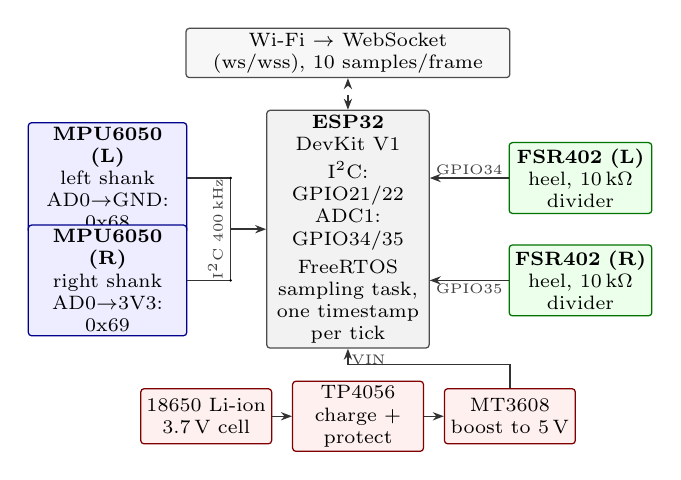
\begin{tikzpicture}[
  font=\scriptsize,
  >={Stealth[length=1.4mm]},
  part/.style={draw=black!70, rounded corners=1.2pt, align=center, inner sep=1.6pt, fill=white, line width=0.45pt},
  imu/.style={part, fill=blue!7, draw=blue!55!black, text width=19mm, minimum height=9mm},
  fsr/.style={part, fill=green!8, draw=green!45!black, text width=17mm, minimum height=9mm},
  pwr/.style={part, fill=red!6, draw=red!50!black, text width=15.5mm, minimum height=7mm},
  wire/.style={line width=0.55pt, draw=black!80},
  lbl/.style={font=\tiny, text=black!75, align=center, inner sep=1pt},
]
\node[part, fill=black!5, text width=19.5mm, minimum height=25mm] (esp) at (0,0)
  {\textbf{ESP32}\\DevKit V1\\[0.8mm]I$^2$C: GPIO21/22\\ADC1: GPIO34/35\\[0.8mm]FreeRTOS\\sampling task,\\one timestamp\\per tick};

\node[imu, anchor=east] (imuL) at ($(esp.west)+(-10mm, 6.5mm)$) {\textbf{MPU6050 (L)}\\left shank\\AD0$\to$GND: 0x68};
\node[imu, anchor=east] (imuR) at ($(esp.west)+(-10mm,-6.5mm)$) {\textbf{MPU6050 (R)}\\right shank\\AD0$\to$3V3: 0x69};

% shared I2C bus
\coordinate (busx) at ($(esp.west)+(-4.5mm,0)$);
\draw[wire] (imuL.east) -- (imuL.east -| busx);
\draw[wire] (imuR.east) -- (imuR.east -| busx);
\draw[wire] (imuL.east -| busx) -- (imuR.east -| busx);
\draw[wire, ->] (busx) -- (esp.west |- busx);
\fill (imuL.east -| busx) circle (0.5pt);
\fill (imuR.east -| busx) circle (0.5pt);
\node[lbl, rotate=90, anchor=south] at ($(busx)+(-0.6mm,0)$) {I$^2$C 400\,kHz};

\node[fsr, anchor=west] (fsrL) at ($(esp.east)+(10mm, 6.5mm)$) {\textbf{FSR402 (L)}\\heel, 10\,k$\Omega$\\divider};
\node[fsr, anchor=west] (fsrR) at ($(esp.east)+(10mm,-6.5mm)$) {\textbf{FSR402 (R)}\\heel, 10\,k$\Omega$\\divider};
\draw[wire, ->] (fsrL.west) -- node[lbl, above]{GPIO34} (fsrL.west -| esp.east);
\draw[wire, ->] (fsrR.west) -- node[lbl, below]{GPIO35} (fsrR.west -| esp.east);

% power chain
\node[pwr, below=5mm of esp, xshift=-18mm] (bat) {18650 Li-ion\\3.7\,V cell};
\node[pwr, right=2.5mm of bat] (chg) {TP4056\\charge + protect};
\node[pwr, right=2.5mm of chg] (bst) {MT3608\\boost to 5\,V};
\draw[wire, ->] (bat) -- (chg);
\draw[wire, ->] (chg) -- (bst);
\draw[wire, ->] (bst.north) |- ($(esp.south)+(0,-2mm)$) -- node[lbl, right, pos=0.3]{VIN} (esp.south);

% wireless link
\node[part, above=4mm of esp, text width=40mm, fill=black!3] (srv) {Wi-Fi $\rightarrow$ WebSocket (ws/wss), 10 samples/frame};
\draw[wire, <->, dashed] (esp.north) -- (srv.south);
\end{tikzpicture}

\caption{Wearable node: one ESP32 samples both shank IMUs (shared I$^2$C bus, distinct addresses) and two heel force sensors in the same tick.}
\label{fig:hw}
\end{figure}

\subsection{Protocol, Provenance and Stream Integrity}
A \emph{hello} frame declares each IMU (side, placement, ranges), each force channel and a per-device key. Provenance is fixed at this handshake, never inferred from data: a registered device presenting its own key is \textsc{live}, the simulator is \textsc{simulated}, anything else is \textsc{unverified}, and only \textsc{live} sessions can become training data. Every packet is checked for ordering, duplicates, gaps, measured sampling rate, jitter, frozen IMUs, saturation and impossible values; clock drift is fitted to the \emph{lower envelope} of arrival times so that network queuing is not mistaken for drift.

\subsection{Per-Wearing Calibration}
At every wearing the device LED guides (1)~a sensor health check, (2)~3\,s of stillness on every IMU, \emph{detected} rather than timed, and (3)~5\,s of slow repetitions. Eight checks follow (connectivity, sampling rate, gravity plausibility, accelerometer baseline, gyroscope bias, force sensor, neutral pose, baseline movement), each graded PASS, WARN or FAIL with stored thresholds. Per IMU the outputs are the gyroscope bias $\vect{b}_\omega$, the neutral gravity direction $\vect{g}_0$ and the principal rotation axis $\vect{u}$; the exact sample windows are stored, so a calibration can be recomputed from raw data.

\subsection{Cloud Platform}
The service uses FastAPI with asynchronous WebSockets over PostgreSQL, and the clinician dashboard is a Next.js application; both run on Vercel, with live messages relayed between instances through PostgreSQL \textsc{listen/notify}. Raw samples are stored losslessly (about 19\,MB per hour) and expire after 30 days unless the patient consents to their use for training. Passwords are Argon2id hashes, access is authorised on the server, model bundles are SHA-256 verified, and the code is covered by 279 back-end and 8 ML tests.

% =====================================================================
\section{Methodology}

\subsection{Mounting-Invariant Features}
One function prepares model input in training and deployment alike: a moving-average anti-alias filter and linear resampling to 25\,Hz, with windows of $W=2$\,s and stride $s=0.5$\,s (response delay $\approx W/2+s=1.5$\,s). For accelerations $\vect{a}_t$ (g) and angular velocities $\boldsymbol{\omega}_t$ ($^\circ$/s) in a window with gravity direction $\hat{\vect{g}}=\bar{\vect{a}}/\lVert\bar{\vect{a}}\rVert$, each IMU is mapped to six channels:
\begin{equation}
\begin{aligned}
&\lVert\vect{a}_t\rVert,\quad \vect{a}_t\!\cdot\!\hat{\vect{g}},\quad \lVert\vect{a}_t-(\vect{a}_t\!\cdot\!\hat{\vect{g}})\hat{\vect{g}}\rVert,\\
&\lVert\boldsymbol{\omega}_t\rVert,\quad \boldsymbol{\omega}_t\!\cdot\!\hat{\vect{g}},\quad \lVert\boldsymbol{\omega}_t-(\boldsymbol{\omega}_t\!\cdot\!\hat{\vect{g}})\hat{\vect{g}}\rVert .
\end{aligned}
\label{eq:inv}
\end{equation}
A rotation $\vect{R}$ of the sensor frame maps $\vect{a}_t\!\mapsto\!\vect{R}\vect{a}_t$ and $\hat{\vect{g}}\!\mapsto\!\vect{R}\hat{\vect{g}}$ and preserves norms and dot products, so all six channels are independent of how the strap is put on. Each channel yields 24 time- and frequency-domain statistics (moments, percentiles, spectral entropy, band energies, autocorrelation), plus jerk RMS.

Invariance discards posture. We restore it relative to the neutral direction $\vect{g}_0$, measured during calibration \emph{in the same sensor frame} and therefore rotating with the sensor:
\begin{equation}
\theta^{n}_t=\arccos\!\left(\vect{a}_t\!\cdot\!\vect{g}_0/\lVert\vect{a}_t\rVert\right),
\label{eq:neutral}
\end{equation}
summarised by its mean, deviation and range, with the acceleration along and angular velocity about $\vect{g}_0$ (8 features). Cross-side correlation, lag and variance-ratio features add 18, for 153 features per IMU and 324 for the bilateral model.

\subsection{Activity Classifier and Pre-Registered Selection}
The nine classes are those the public datasets share (lying, sitting, standing, walking, stairs up/down, running, cycling, other exercise); there is deliberately no squat class, because no public dataset contains one, and the prescribed exercise is known from the session. Candidates were a random forest (RF; 200 trees, class-balanced)~\cite{breiman2001,pedregosa2011}, histogram gradient boosting (HGB)~\cite{ke2017}, the RF with device-like augmentation, and three deep models: a 1D CNN, a CNN-LSTM~\cite{ordonez2016} and a CNN with a PAMAP2-pretrained encoder. The rule, written before any result was inspected, takes for each feature-model family the shortest window within 0.01 macro-F1 of its best, then the highest macro-F1 with a rotation drop $\le0.03$ and 95th-percentile latency $\le50$\,ms (ties within 0.01 go to the smaller model); a deep model is adopted only if it is $\ge0.02$ better and meets the same limits. Predictions with top probability below $\tau=0.3$ are reported as \textsc{low\_confidence}, never as the answer.

\subsection{Segment Tilt and Range-of-Motion Proxy}
With one IMU per leg there is no knee angle, so RehabSense reports a segment tilt and, per repetition, its range as a \emph{range-of-motion (ROM) proxy}. Following the axis-identification idea of~\cite{seel2014}, $\vect{u}$ is the first right-singular vector of the gyroscope samples from the calibration movement. The accelerometer tilt $\theta^{a}_t$ is the signed angle between $\vect{g}_0$ and $\vect{a}_t$ projected onto the plane normal to $\vect{u}$, fused by a complementary filter~\cite{mahony2008}:
\begin{equation}
\theta_t=\alpha\left(\theta_{t-1}+(\boldsymbol{\omega}_t\!\cdot\!\vect{u})\,\Delta t\right)+(1-\alpha)\,\theta^{a}_t,\qquad \alpha=0.98.
\label{eq:tilt}
\end{equation}
When $\vect{g}_0$ is nearly parallel to $\vect{u}$, gravity carries no tilt information; the estimate becomes gyroscope-only with a slow leak and is flagged.

\subsection{Repetitions, Asymmetry and Movement Quality}
Repetitions are segmented by peak detection on the tilt (gait cycles for walking). Left and right are compared through normalised differences
\begin{equation}
d(L,R)=\lvert L-R\rvert/\max(\lvert L\rvert,\lvert R\rvert)\in[0,1]
\label{eq:nd}
\end{equation}
of dynamic acceleration RMS, angular-velocity RMS and 95th percentile, ROM proxy, waveform dissimilarity and timing (relative to the expected relation: in phase for squats, half a cycle apart for walking). The asymmetry score $A$ is the mean of the available components; components below their noise floor are dropped, and a one-sided stream returns \textsc{single\_side} instead of a score---a missing side is never mirrored.

The MQI combines six components $c_i\in[0,1]$: symmetry ($1-A$), ROM proxy relative to the patient's baseline (capped at 1), temporal consistency ($1-$ coefficient of variation of repetition durations), smoothness (SPARC~\cite{balasubramanian2015} mapped from $[-7,-1.5]$ to $[0,1]$), force-peak consistency and repetition-shape correlation:
\begin{equation}
\mathrm{MQI}=100\,\textstyle\sum_{i\in\mathcal{A}}w_i c_i\big/\sum_{i\in\mathcal{A}}w_i ,
\label{eq:mqi}
\end{equation}
over the available set $\mathcal{A}$. With no labels to fit them, the weights are equal---an assumption, not a finding. The definition is frozen by a SHA-256 hash, and MQIs from different component sets are never compared.

% =====================================================================
\section{Experimental Setup}

\textbf{Datasets.} \emph{Daily and Sports Activities}~\cite{altun2010} provides 8 subjects with Xsens units on both legs \emph{recorded simultaneously}---real bilateral data---and trains the bilateral model. \emph{PAMAP2}~\cite{reiss2012} contributes 9 subjects with an ankle IMU to the single-IMU model and to encoder pretraining. \emph{UCI HAR}~\cite{anguita2013}, used here in a 561-feature form without raw signals, is a tooling check on its official split (macro-F1: RF 0.923, HGB 0.936) and is not deployable. A single-IMU recording is never mirrored into a fake left--right pair, and one standing segment per subject is reserved to emulate calibration and excluded from evaluation.

\textbf{Protocol.} Splits are GroupKFold(4) by subject, with windows cut inside recordings and out-of-fold predictions pooled; macro-F1 is the primary metric~\cite{saeb2017}. Robustness is measured on test folds after a random 3D rotation of each sensor, 3$\times$ noise, $\pm3^\circ$/s gyroscope bias, $\pm5$\% accelerometer gain error and a 5\% clock error. Transfer is measured between the Daily and Sports leg sensors and the PAMAP2 ankle sensor. Latency is single-window feature extraction plus prediction on one laptop CPU thread (200 runs).

\textbf{Verification.} Public windows are replayed as quantised, jittered 100\,Hz device streams through the server's inference path and its full processor; a dual-IMU simulator straps each IMU at a random orientation and generates five exercises with known ROM, injected left-side deficits (0--0.6) and injected faults.

% =====================================================================
\section{Results and Discussion}

\subsection{Mounting Invariance}
Fig.~\ref{fig:ablation} isolates the representation. Raw-axis features score highest on the original mounting (0.943) but collapse to 0.199 once the test sensors are rotated, exactly what a re-attached strap does. Invariant channels alone are immune to rotation but lose posture (0.829) and are fragile under noise (0.699). Adding neutral-pose posture restores 0.921, unchanged under rotation and nearly so under 3$\times$ noise (0.915).

\begin{figure}[t]
\centering
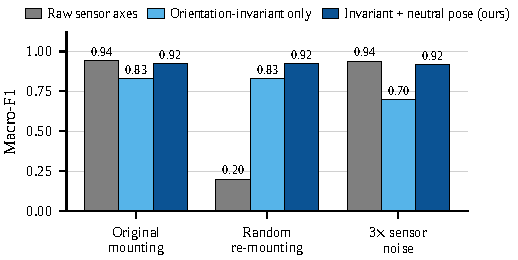
\includegraphics[width=\columnwidth]{fig_orientation_ablation.pdf}
\caption{Feature-set ablation (bilateral RF, 2\,s windows, subject-independent macro-F1) under the original mounting, random re-mounting and 3$\times$ sensor noise.}
\label{fig:ablation}
\end{figure}

\subsection{Model Selection}
Table~\ref{tab:bench} reports the benchmark. HGB is most accurate (0.945 at 3\,s) but needs 156\,ms per window, three times the budget. The RF at 2\,s (0.921) lies within 0.01 of its family's best and responds faster, so the rule selects it; the augmented RF ties and loses on size (15.4 vs.\ 9.6\,MB) despite better noise robustness. The deep models trail by 0.023--0.051, although PAMAP2 pretraining lifts the CNN by 0.027, keeping it the candidate for force fusion once device data exist.

\begin{table}[t]
\caption{Subject-independent benchmark (Daily \& Sports, 9 classes)}
\label{tab:bench}
\centering
\scriptsize
\setlength{\tabcolsep}{3.4pt}
\begin{tabular}{@{}llccccr@{}}
\toprule
Model & Features & $W$ (s) & F1 & Rot. & 3$\times$noise & p95 (ms) \\
\midrule
RF & raw axes (control) & 2 & 0.943 & \textbf{0.199} & 0.939 & 5.4 \\
RF & invariant only & 2 & 0.829 & 0.829 & 0.699 & 5.0 \\
\textbf{RF$^\star$} & \textbf{inv.\ + neutral} & \textbf{2} & \textbf{0.921} & \textbf{0.921} & \textbf{0.915} & \textbf{12.9} \\
RF & inv.\ + neutral & 3 & 0.929 & 0.929 & 0.919 & 5.3 \\
RF & + device aug. & 2 & 0.921 & 0.921 & 0.919 & 6.2 \\
HGB & inv.\ + neutral & 3 & 0.945 & 0.945 & 0.852 & 156.4 \\
1D CNN & 9 ch./IMU seq. & 2 & 0.871 & 0.871 & 0.868 & 0.4 \\
CNN-LSTM & 9 ch./IMU seq. & 2 & 0.896 & 0.896 & 0.893 & 0.9 \\
CNN, pretr. & 9 ch./IMU seq. & 2 & 0.898 & 0.898 & 0.900 & 0.3 \\
\midrule
RF, 1 IMU & inv.\ + neutral & 2 & 0.895 & 0.895 & 0.859 & 5.0 \\
\bottomrule
\end{tabular}\\[2pt]
\parbox{\columnwidth}{\scriptsize $^\star$Deployed. F1: macro-F1; Rot.: after random sensor rotation. Single-IMU model: each Daily \& Sports leg plus the PAMAP2 ankle. Transfer: Daily \& Sports$\to$PAMAP2 0.241, reverse 0.153.}
\end{table}


\subsection{Per-Class Behaviour and Selective Prediction}
Cycling, running, standing and lying exceed 0.99 recall (Fig.~\ref{fig:cm}). The residual errors are interpretable: a quarter of sitting windows are labelled lying, the posture pair one segment per leg separates least well, and walking and stair windows drift toward \emph{other exercise}, which contains stepper and cross-trainer movements. At $\tau=0.3$ the model answers 99.99\% of windows with 91.8\% accuracy; $\tau=0.7$ raises accuracy to 97.3\% on 80.2\% of windows. The threshold must be re-derived on device data, where probabilities are not calibrated.

\begin{figure}[t]
\centering
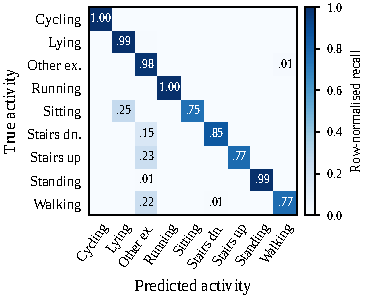
\includegraphics[width=\columnwidth]{fig_confusion.pdf}
\caption{Row-normalised confusion matrix of the deployed model (out-of-fold, 60{,}424 windows, 8 held-out subjects).}
\label{fig:cm}
\end{figure}

\subsection{Domain Gap and Train--Serve Parity}
Cross-dataset transfer collapses to 0.241 and 0.153 macro-F1, measuring what a change of sensor and placement costs; public-data scores are therefore pretraining evidence, not device accuracy. The device path itself is faithful: device-format replay reproduces the training-path prediction for 98.4\% of 800 windows, and the full processor agrees with the labels on 95.6\% of 1{,}152 windows---integrity checks on subjects seen in training, not generalisation estimates.

\subsection{Movement Metrics in Simulation}
Against simulated ground truth, the tilt is within 2.5$^\circ$ (median) under random strap orientations, repetition counts fall within 1--3 of the simulated cycles (incomplete cycles are excluded), and all four injected faults (packet loss, IMU dropout, frozen IMU, impossible values) are detected. The ROM proxy is within $\pm1.5$\% for the four repetitive exercises but underestimates walking by 9.4\%, plausibly because heel-strike accelerations violate the quasi-static assumption behind the accelerometer tilt. The asymmetry score rises monotonically with the injected deficit and the MQI falls from 96.0 to 80.8 (Fig.~\ref{fig:sim}), with a repeatability of $\pm0.08$ over ten seeds. Removing the right IMU moves the MQI from 96.0 to 95.2 only because its symmetry term disappears---which is why scores from different component sets are never compared.


\begin{figure}[t]
\centering
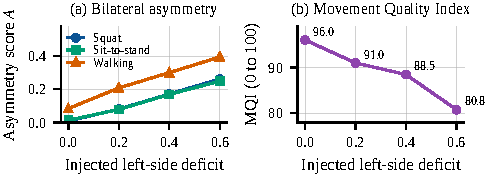
\includegraphics[width=\columnwidth]{fig_simulator.pdf}
\caption{Simulator characterisation versus injected left-side deficit: (a) asymmetry score; (b) MQI (mean $\pm$ SD, 3 seeds).}
\label{fig:sim}
\end{figure}

\subsection{System Performance}
On the server, features plus prediction take 4.7\,ms per window (median), negligible beside the 1.5\,s windowing delay. The loaded forests, however, occupy about 220\,MB (bilateral) and 460\,MB (single-IMU), so edge inference on the ESP32 would need a compact model such as a few shallow trees or an int8 CNN.

% =====================================================================
\section{Limitations and Future Work}
RehabSense is a research prototype, not a medical device. Its activity model is validated on public data only; no physical-device recording has yet been evaluated, and the transfer results predict a substantial drop until the model is adapted. The ROM proxy is a segment tilt, not a knee angle; the force channels are an uncalibrated load proxy; and the MQI weights and SPARC bounds are assumptions characterised only on idealised kinematics. The next stage is an ethics-approved pilot on a registered device: consented participants recorded on two days with re-strapping, therapist-labelled repetitions and quality ratings, zero-shot then fine-tuned leave-one-subject-out evaluation, the ROM proxy against a goniometer or optical reference, and MQI reliability (intraclass correlation) against therapist ratings. By lowering the cost of objective home monitoring, the work supports UN Sustainable Development Goals~3 (good health and well-being) and~9 (industry, innovation and infrastructure).

\section{Conclusion}
RehabSense pairs a US\$18 bilateral wearable with an analytics pipeline that is robust to how patients put it on and explicit about what its numbers mean. Measuring posture against a calibrated neutral pose reconciles orientation invariance with posture recognition (macro-F1 0.921, unchanged under re-mounting, against 0.199 for raw axes); a pre-registered rule selects a model within a real-time budget; and replay shows that the device path reproduces the training path. The platform is ready for the pilot study that will supply its first hardware and clinical evidence.

\section*{Acknowledgment}
The authors thank the Department of Computer Engineering, Vishwakarma Institute of Technology, Pune, for supporting this work, and the creators of the Daily and Sports Activities, PAMAP2 and UCI HAR datasets for releasing their data.

\IEEEtriggeratref{14}
\bibliographystyle{IEEEtran}
\bibliography{references}

\end{document}
